
Die Informatik umfasst eine Vielzahl unterschiedlicher Fachgebiete mit teils stark variierenden Schwerpunkten. 
Dazu zählen unter anderem die Web- und Anwendungsentwicklung sowie der Bereich der IT-Sicherheit und viele weitere Disziplinen. 
Im Rahmen dieser Arbeit liegt der Fokus auf dem speziellen Teilbereich der Embedded-Softwareentwicklung.

In diesem Kapitel werden die grundlegenden fachlichen und technischen Konzepte vermittelt, die zum Verständnis der weiteren Inhalte erforderlich sind.
% Ablauf des Kapitels
Zu Beginn wird eine Einführung in das Themenfeld der Embedded-Systeme gegeben, um ein klares Verständnis dafür zu schaffen, welche Unterschiede diesen Bereich kennzeichnen und wie er sich von anderen Teilgebieten der Informatik unterscheidet.
Darauffolgend werden zentrale Begriffe und Konzepte erläutert, die in der Embedded-Entwicklung eine signifikante Rolle spielen, wie beispielsweise Register, Ports, Peripherieansteuerung und hardwarenahe Programmierung.
Darüber hinaus wird technisches Hintergrundwissen vermittelt, das für das Verständnis der späteren Implementierungsschritte und der Architekturentscheidungen von Relevanz ist.

%Das Ziel dieses Kapitels besteht darin, eine solide Wissensbasis zu schaffen, auf der die Analyse bestehender Lösungen sowie die Entwicklung einer eigenen Treiber-API aufbauen können.
\section{Hardware}
\subsection{Eingebettete Systeme}
Bevor auf die Entwicklung eingebetteter Systeme eingegangen werden kann, ist zunächst zu klären, worum es sich bei diesen Systemen handelt.
Der Begriff \emph{Embedded System} (deutsch: eingebettetes System) bezeichnet ein Computersystem, das aus Hardware und Software besteht und fest in einen übergeordneten technischen Kontext integriert ist. 
Typischerweise handelt es sich dabei um Maschinen, Geräte oder Anlagen, in denen das eingebettete System spezifische Steuerungs-, Regelungs- oder Datenverarbeitungsaufgaben übernimmt.
Ein wesentliches Merkmal eingebetteter Systeme besteht darin, dass sie nicht als eigenständige Recheneinheiten agieren, sondern als integraler Bestandteil eines übergeordneten Gesamtsystems dienen.
In der Regel operieren sie im Hintergrund und sind nicht direkt mit den Benutzern verbunden. In einigen Fällen erfolgt die Interaktion automatisch, in anderen durch Eingaben des Nutzers.

\paragraph{Definition:}
Ein Embedded System ist ein spezialisiertes, in sich geschlossenes Computersystem, das für eine klar definierte Aufgabe innerhalb eines übergeordneten technischen Systems konzipiert wurde.

\vspace{6 mm}

Die Entwicklung von Software für eingebettete Systeme ist mit besonderen Anforderungen verbunden, die sich signifikant von denen unterscheiden, die etwa in der Web- oder Anwendungsentwicklung üblich sind.
Es ist von besonderer Bedeutung, hardwarenahe Aspekte zu berücksichtigen, da die Software unmittelbar mit der zugrunde liegenden Mikrocontroller-Hardware interagiert.
Ein zentraler Aspekt dabei ist die Integration geeigneter Treiber für die jeweilige Mikrocontroller-Architektur.
Die betreffenden Treiber beinhalten Funktionen, welche den Zugriff auf die Hardware mittels sogenannter Register erlauben.
Register sind spezifische Speicherbereiche innerhalb des Mikrocontrollers, welche eine unmittelbare Manipulation des Hardware-Verhaltens ermöglichen.
Durch das gezielte Setzen oder Auslesen einzelner Bits in diesen Registern ist es möglich, beispielsweise Sensorwerte zu erfassen (z. B. das Drücken eines Tasters) oder Ausgaben zu erzeugen (z. B. das Anzeigen eines Textes auf einem Display).




\subsection{Microcontroller Unit (MCU)}
Ein Mikrocontroller ist ein vollständig auf einem einzigen Chip realisierter Mikrocomputer, der neben dem eigentlichen Prozessor (CPU) auch sämtliche für den Betrieb notwendigen Komponenten integriert. 
Zu den Komponenten eines solchen Systems zählen in der Regel Programmspeicher (Flash), Datenspeicher (\gls{ram}), digitale Ein- und Ausgänge (\gls{gpio}), Timer, Kommunikationsschnittstellen (wie \gls{uart}, \gls{spi}, \gls{i2c}, \gls{can}) sowie in vielen Fällen analoge Peripheriekomponenten wie Analog/Digital-Wandler oder Pulsweitenmodulation-Einheiten.

Mikrocontroller werden für spezifische Steuerungs- und Regelungsaufgaben konzipiert und finden typischerweise Anwendung in eingebetteten Systemen, wie beispielsweise Haushaltsgeräten, Fahrzeugsteuerungen, Industrieanlagen oder IoT-Geräten. 
Die Geräte zeichnen sich durch einen geringen Energieverbrauch, eine kompakte Bauform, niedrige Kosten und eine direkte Hardwareansteuerung aus. 
Im Vergleich zu Mikroprozessoren sind für den Grundbetrieb von Mikrocontrollern keine externen Komponenten erforderlich, was besonders kompakte und zuverlässige Systemlösungen ermöglicht.


%\subsection*{Hardware Architektur}
%- CISC vs. RISC
%
%- Cortex Familie




\subsection{Peripherie}
Unter dem Begriff der \emph{Peripherie} versteht man im Kontext der Embedded-Softwareentwicklung sämtliche Ein- und Ausgabeschnittstellen, die eine Interaktion des Mikrocontrollers mit seiner Umwelt ermöglichen.
Peripheriegeräte stellen die Verbindung zwischen der digitalen Rechenlogik des Mikrokontrollers und der realen Welt her.
Sie ermöglichen die Erfassung, Verarbeitung und Ausgabe physikalischer Signale wie Temperatur, Licht oder der Betätigung eines Tasters.
Ein moderner Mikrocontroller, wie etwa ein STM32, ist bereits mit einer Vielzahl an integrierten Peripherieeinheiten ausgestattet, darunter digitale Ein-/Ausgänge (GPIOs), serielle Kommunikationsschnittstellen (UART, SPI, I2C, CAN), analoge Wandler (ADC, DAC), Timer oder PWM-Module. 
Die als \emph{On-Chip} bezeichneten Komponenten sind integraler Bestandteil des Mikrocontrollers und können über zugehörige Register programmiert und gesteuert werden.
Zusätzlich zur integrierten Peripherie besteht die Möglichkeit, über die physischen Pins des Mikrocontrollers auch externe Peripheriegeräte anzuschließen. 
Die Verbindung erfolgt in der Regel mittels Steckverbindungen, wie etwa Jumper-Kabeln, Steckbrücken, Pin-Headern oder speziellen Anschlussleisten auf Entwicklungsboards. 
In der Regel werden zu diesem Zweck Steckbretter (Breadboards) oder Lochrasterplatinen verwendet, um eine übersichtliche und flexible Verdrahtung zu gewährleisten. 
Externe Bauteile, wie etwa Sensoren (Temperatursensor), Aktoren (LED), Displays oder Speicherbausteine, werden über gängige Schnittstellen wie I2C, SPI, UART oder digitale GPIOs mit dem Mikrocontroller verbunden.
Die Kommunikation mit externen Geräten wird durch die Peripheriemodule des Mikrocontrollers realisiert. 
Für den zuverlässigen Betrieb sind in der Regel spezifische Softwaretreiber erforderlich, die die Initialisierung, Datenübertragung und gegebenenfalls die Fehlerbehandlung übernehmen.

% TODO: chap3 Peripherie: Parallel/Seriell; synchron/asynchron; für alle nochmal drüber gehen
\subsubsection*{General Purpose Input Output}
Der Begriff "General Purpose Input/Output" (GPIO) bezeichnet universelle, digitale Pins eines Mikrocontrollers, die flexibel als Eingang oder Ausgang konfiguriert werden können.
Sie stellen die grundlegendste Form der Interaktion mit der Außenwelt dar und gestatten die Erfassung externer digitaler Signale, z.B. von Tastern oder Sensoren, sowie die Erzeugung entsprechender Signale etwa zur Steuerung von LEDs oder Relais.
Grundsätzlich können GPIOs flexibel als Eingang oder Ausgang verwendet werden.
Typischerweise erfolgt die Konfiguration solcher Embedded-Systeme statisch während der Initialisierung, entweder automatisch durch Codegeneratoren wie STM32CubeMX oder manuell in der Startkonfiguration der Firmware.
Obwohl eine Änderung der GPIO-Funktionalität zur Laufzeit technisch möglich wäre, wird dies in der Praxis häufig vermieden, um ein deterministisches und stabiles Systemverhalten zu gewährleisten.
In der praktischen Anwendung bilden sie die Grundlage für einfache Steuerungs- und Überwachungsaufgaben und sind daher von zentraler Bedeutung für die hardwarenahe Embedded-Programmierung.

\subsubsection*{Serial Peripheral Interface}
Die Schnittstellen des \emph{Serial Peripheral Interface} (SPI) ist ein synchrones, serielles Kommunikationsprotokoll, das insbesondere für die schnelle und effiziente Datenübertragung über kurze Distanz zwischen einem Master- und einem oder mehreren Slave-Geräten eingesetzt wird. 
Die primäre Aufgabe des Protokolls besteht in der Verbindung von \gls{mcu}s mit integrierten oder externen Komponenten, zu denen unteranderem  Sensoren, Speicher, Aktoren sowie Displays zählen.
SPI arbeitet synchron, d.h. Sender und Empfänger teilen sich ein gemeinsames Taktsignal.
Der Master ist derjenige, der diesen Takt vorgibt und bereitgestellt.
Dadurch wird eine präzise, zeit-sensitive Übertragung ermöglicht. 
Die zentrale Eigenschaft von \gls{spi}, die das gleichzeitige Senden und Empfangen ermöglicht ist die Unterstützung der Voll-Duplex-Kommunikation.
% TODO: SPI: Quellenverweise einfügen.
Der \gls{spi}-Bus verwendet meistens vier physikalische Leitungen:
\begin{itemize}
	\item \gls{miso} / \gls{cipo} für die Kommunikation vom Master zu den Peripheriegeräten (Slaves).
	\item \gls{mosi} / \gls{copi} für die Kommunikation von den Peripheriegeräten zum Master.
	\item \gls{ss} / \gls{cs} für die Auswahl des gewünschten Peripheriegerätes.
	\item \gls{sclk} als Taktleitung, die den vom Master vorgegebenen Takt enthält.
\end{itemize}

In der Regel dient der Mikrokontroller als Master, der den Datenfluss steuert.
Mittels des Slave-Signals ist es der \gls{mcu} möglich, gezielt Slaves anzusprechen.
Dabei ist darauf zu achten, dass jeweils nur ein Slave die Kommunikation aktiv durchführen darf, um eine Kollision auf Bus zu vermeiden.

\gls{spi} zeichnet sich im Vergleich zu anderen seriellen Protokollen wie \gls{i2c} durch eine vereinfachte Implementierung und eine deutlich höhere Datenübertragungsrate aus. 
Allerdings fehlen eine standardisierte Adressierung und Fehlerprüfung, was den Einsatz auf kurze Distanzen und überschaubare Topologien begrenzt. 


\subsubsection*{Universal Asynchronous Receiver Transmitter}
Der \emph{Universal Asynchronous Receiver Transmitter} (UART) ist ein asynchrones Kommunikationsprotokoll, das insbesondere für die serielle, asynchrone Punkt-zu-Punkt-Kommunikation zwischen zwei Geräten eingesetzt wird. 
Das Protokoll eignet sich für verschiedene Anwendungsbereiche, darunter als Debugging-Schnittstelle, der Kommunikation von Sensoren, GPS-Modulen sowie die Kommunikation mit Computern über USB-zu-Seriell-Wandler. 
Im Gegensatz zu synchronen Schnittstellen wie SPI ist für UART kein gemeinsames Taktsignal erforderlich.
Die Datenübertragung passiert hier asynchron über zwei Leitungen: eine für das Senden (Transmitter TX) und eine für das Empfangen (Receiver RX).
Die Synchronisation basiert auf einer zuvor festgelegten Baudrate (Bits pro Sekunde), die von beiden Geräten unabhängig voneinander eingehalten werden muss.
Die Kommunikation, d.h. die Datenübertragung erfolgt in sogenannten Frames. Ein typisches \gls{uart}-Frame besteht aus:
% TODO: UART: Quellenverweise einfügen
\begin{itemize}
	\item \textbf{Startbit}, das den Begin eines Datenframes signalisiert,
	\item \textbf{Datenframe}, bestehend aus fünf bis acht Bits,
	\item \textbf{Paritätsbit}, das einer einfacheren Fehlererkennung dient und
	\item \textbf{Stopbit}, das das Ende des Datenframes markiert.
\end{itemize}

In Abhängigkeit von der Implementierung unterstützt UART Simplex-, Halbduplex- und Vollduplex-Kommunikation. 
In einer Vielzahl von Mikrocontrollern ist UART als Hardwaremodul integriert, wodurch die serielle Kommunikation effizient und mit minimalem Softwareaufwand realisiert werden kann. 
Dennoch erfordert die korrekte Konfiguration – insbesondere die Wahl der Baudrate, des Paritätsmodus und der Anzahl von Stoppbits – besondere Sorgfalt, da Abweichungen zu Datenverlust oder Kommunikationsfehlern führen können.
Ein weiterer Vorteil von UART ist seine Einfachheit in Aufbau und Handhabung: Es werden lediglich zwei Leitungen benötigt. 
Die Kommunikation ist prinzipiell auf zwei Geräte beschränkt (Punkt-zu-Punkt-Verbindung), da UART keine native Unterstützung für Bussysteme mit mehreren Teilnehmern bietet.

\subsubsection*{Controller Area Network}
Das \emph{Controller Area Network} (CAN) ist ein robustes, serielles, asynchrones Bussystem, das insbesondere in der Automobilindustrie eine weite Verbreitung findet. 
Es ermöglicht eine zuverlässige Kommunikation zwischen mehreren Steuergeräten (Nodes), auch unter schwierigen elektromagnetischen Bedingungen. 
Der Einsatz von CAN in sicherheitskritischen Anwendungen beruht auf zwei wesentlichen Eigenschaften: 
\begin{itemize}
	\item der prioritätsbasierten Arbitrierung
	\item der integrierten Fehlererkennung
\end{itemize}
 
Diese Eigenschaften gewährleisten eine hohe Ausfallsicherheit.
Die CAN-Technologie basiert auf einem \emph{shared medium} mit Bus-Topologie, bei der alle Teilnehmer über zwei Leitungen mit einander verbunden sind.
Jedes angeschlossene Gerät ist dazu befähigt, Nachrichten auf den Bus zu senden und alle Nachrichten auf dem Bus zu empfangen, allerdings verarbeitet jeder Knoten lediglich die Informationen, die für ihn relevant sind. 
Eine zielgerichtete Adressierung von Empfängern ist im Protokoll nicht vorgesehen.
Stattdessen findet bei CAN ein nachrichtenbasiertes Kommunikationsmodell Anwendung, bei dem jede Nachricht durch eine eindeutige Identifier (ID) gekennzeichnet ist. 
Diese ID dient nicht der Beschreibung des Absenders oder Empfängers der Nachricht, sondern gibt Aufschluss über den Inhalt der Nachricht, z.B. ob es sich um Geschwindigkeit, das Drehmoment oder die Sensordaten handelt.
Es ist grundsätzlich möglich, dass mehrere Knoten auf dieselbe Nachricht reagieren.

Ein wesentliches Merkmal ist die prioritätsbasierte Arbitrierung. 
Jeder Knoten hat die Möglichkeit, eine Nachricht gleichzeitig zu senden. 
Das Protokoll verwendet ein bitweises Arbitrierungsverfahren. 
Nachrichten mit einer niedrigeren ID (höhere Priorität) durchdringen das System automatisch, ohne dass es zu Kollisionen oder Datenverlust kommt.
Dieses Verfahren zeichnet sich durch seine besondere Effizienz aus und ist in der Lage, Echtzeitanforderungen zu erfüllen.

Obwohl CAN asynchron ist, d. h. jeder Knoten hat seinen eigenen Takt, erfolgt die Synchronisation der Kommunikation durch ein fein abgestimmtes Zeitraster.
Ein Bit lässt sich in sogenannte Zeitquanten unterteilen. 
Diese sind in mehrere Segmente unterteilt, nämlich Synchronisation, Propagation, Phase 1 und Phase 2. 
Der Abtastzeitpunkt befindet sich zwischen Phase 1 und Phase 2.


\section{Software}

\subsection{Architektur- und Designmuster}
Unter Architektur, speziell \emph{Softwarearchitektur} versteht man den Prozess eine allgemeine Struktur für ein Softwaresystem zu erstellen.
Helmut Balzert definiert den Begriff als ''eine strukturierte oder hierarchische Anordnung der Systemkomponenten sowie Beschreibung ihrer Beziehungen'' \cite{balzert2011softwaretechnik2}.
In diesem Prozess gilt es, die Komponenten in eine grobe (high-level) Gliederung zu bringen.
Im Kontext der Embedded Systeme und Entwicklung und speziell dieser Arbeit, wird sich primär mit der \emph{Schichtenarchitektur} befasst.

Bei diesem Architekturmuster wird das gesamte System in Schichten unterteilt, die  Handlungsbereiche darstellen.
Diese Schichten funktionieren so, dass sie nur mit der direkt anliegenden tieferen Schicht kommunizieren können.
Das bedeutet eine Schicht $n$ kann nur mit der Schicht $n-1$ kommunizieren und ist von dieser abhängig.
Schicht $n-1$ bietet dabei die entsprechenden Funktionen für Schicht $n$.
Umgekehrt gilt diese Abhängigkeit aber nicht.

Im Embedded Bereich lassen sich die Schichten wie folgt beschreiben:

\paragraph{Die Anwendungsschicht/Application Layer}
dient als oberste Schicht.
Diese besteht aus allen Dateien, Funktionen und Klassen, die nicht direkt mit den auf Hardwareebene liegenden Registern zu tun haben; so z.B. Hilfsfunktionen.
Stattdessen werden die Funktionen der nächst tieferen Schicht verwendet.

\paragraph{Die Mittelschicht/Middleware}
als optionale zweite Schicht, befasst sich mit möglichen Zusatzfunktionen wie USB, Netzwerkanschlüsse (WLAN), Bluetooth oder IoT (Internet of Things) oder \gls{api}-Funktionen.
Sie dient als verteilende Zwischenschicht zwischen der Programm und der Abstraktionsschicht der Hardware.

\paragraph{Ein Betriebssystem} ist eine weitere ptionale Schicht.
Optional in dem Sinn, das ein Embedded System nicht zwingend eine Betriebssystem benötigt.
Ohne das Betriebssystem werden direkt die Pins, d.h. die Hardware angesprochen und programmiert; z.B. wenn in kleinem Schaltkreis nur ein Schalter, mit dem ein Signal ein oder ausgeschalten werden soll, und eine LED, die mit dem Schaltersignal leuchtet oder nicht, verbaut sind.
Wird ein Betriebssystem eingesetzt bringt das funktionale Erweiterungen mit sich, wie Multitasking oder besseres Zeitmanagement.
Des weiteren muss bei mit einem OS (Operating System) auf die verfügbaren Ressourcen geachtet werden, da der Speicher bei Mikrokontrollern begrenzt ist.

\paragraph{Die Hardwareabstraktionsschicht} (\gls{hal}) befindet sich unter der Middleware bzw. unter dem Betriebssystem.
Gibt es keine zusätzlichen Funktionen in der Middlewareschicht und wird bare-metal entwickelt kann aus der Applikation direkt auf die hier gelagerten Funktionen zugreifen.
Wie dieser direkte Zugriff auf die Abstraktionsschicht aussieht ist in Code \ref{lst:stm32_mx_gpio_init} % TODO: GPIO Code stm32clean
zu sehen.

\begin{lstlisting}[language=C, caption={Funktion zur Initialisierung der GPIO-Pins aus einem STM32-Projekt.}, label={lst:stm32_mx_gpio_init}]
int main(void)
{

  HAL_Init();
  SystemClock_Config();
  MX_GPIO_Init();
  
  while (1){ ... } 
}

	static void MX_GPIO_Init(void)
{
  GPIO_InitTypeDef GPIO_InitStruct = {0};

  /* GPIO Ports Clock Enable */
  __HAL_RCC_GPIOC_CLK_ENABLE();
  __HAL_RCC_GPIOF_CLK_ENABLE();
  __HAL_RCC_GPIOA_CLK_ENABLE();

  /*Configure GPIO pin Output Level */
  HAL_GPIO_WritePin(LEDextern_GPIO_Port, LEDextern_Pin, GPIO_PIN_RESET);

  /*Configure GPIO pins : VCP_USART2_TX_Pin VCP_USART2_RX_Pin */
  GPIO_InitStruct.Pin = VCP_USART2_TX_Pin|VCP_USART2_RX_Pin;
  GPIO_InitStruct.Mode = GPIO_MODE_AF_PP;
  GPIO_InitStruct.Pull = GPIO_NOPULL;
  GPIO_InitStruct.Speed = GPIO_SPEED_FREQ_LOW;
  GPIO_InitStruct.Alternate = GPIO_AF1_USART2;
  HAL_GPIO_Init(GPIOA, &GPIO_InitStruct);

  /*Configure GPIO pin : LEDextern_Pin */
  GPIO_InitStruct.Pin = LEDextern_Pin;
  GPIO_InitStruct.Mode = GPIO_MODE_OUTPUT_PP;
  GPIO_InitStruct.Pull = GPIO_NOPULL;
  GPIO_InitStruct.Speed = GPIO_SPEED_FREQ_LOW;
  HAL_GPIO_Init(LEDextern_GPIO_Port, &GPIO_InitStruct);
}
\end{lstlisting}

Aus der \texttt{int main(void)}, der Hauptfunktion wird die Funktion \texttt{static MX\_GPIO\_Init(void)} zur Initialisierung der Pins aufgerufen.
Am Ende dieser Funktion sieht man \texttt{HAL\_GPIO\_Init(GPIO\_Port, \&GPIO\_InitStruct)}.
Diese Funktion ist Teil der Hardwareabstraktionsschicht, auf die hier ohne weitere Zwischenschicht oder Betriebssystem zugegriffen wird.

\paragraph{Die Treiberschicht} 
ist die letzte Ebene vor der Hardwareschicht.
Diese Schicht arbeitet eng mit der Abstraktionsschicht zusammen.
Sie enthält neben den Low-Level-Treibern, die direkten Zugriff auf die Register haben, den in Assembler geschriebenen Startupcode und Initialisierungsroutinen.


\begin{itemize}
	\item Design Patterns
\end{itemize}


\subsection{Application Programming Interface}
\begin{itemize}
	\item Was ist eine API?
	\item Was kann eine API?
	\item Wie wird eine API umgesetzt?
\end{itemize}




\subsection{CMake}
CMake ist ein plattformübergreifendes Open-Source-Werkzeug zur Automatisierung des Buildprozesses in der Softwareentwicklung
Der sogenannte Metabuild-Generator (\autoref{fig:cmake_generators}) dient als eine Art universeller Konfigurator, der mithilfe Konfigurationsdateien, den \texttt{CMakeLists.txt}-Dateien, spezifische Build-Systeme für eine Vielzahl unterschiedlicher Plattformen und Entwicklungsumgebungen generiert.
Unter diesen Build-Systemen finden sich beispielsweise Makefiles für Unix/Linux, Projektdateien für Visual Studio oder Xcode.

\begin{figure}[H]
	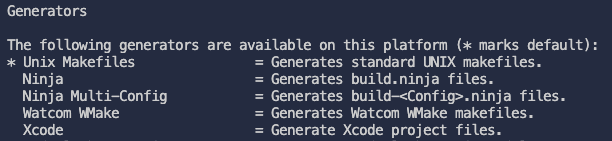
\includegraphics[width=\textwidth]{cmake_generators.png}
	\caption{Ausschnitt einer Liste von verfügbaren Generatoren.}
	\label{fig:cmake_generators}
\end{figure}

Ein wesentlicher Vorteil von CMake liegt in der Trennung von Quell- und Build-Verzeichnissen, was sogenannte Out-of-Source-Builds ermöglicht.
Diese Vorgehensweise trägt zur Schaffung einer übersichtlichen Projektstruktur bei und vereinfacht die Verwaltung von Build-Artefakten.
Zusätlich fördert CMake die hierarchische Strukturierung von Projekten mittels der Implementierung von modularen CMakeLists.txt-Dateien in Unterverzeichnissen.
Dieser Ansatz steigert die Wartbarkeit und Skalierbarkeit komplexer Softwareprojekte.

\subsection{Make und Makefiles}
Make ist ein traditionelles Werkzeug zur Automatisierung von Build-Prozessen, das sogenannte Makefiles zur Steuerung dieser Prozesse einsetzt.
Die Makefiles definieren Regeln, mit deren Hilfe der Quellcode, abhängig davon ob sich etwas im Code geändert hat, kompiliert und verlinkt wird.
Make findet für gewöhnlich Anwendung in der direkten Steuerung von Kompilierungsprozessen.
 Es besteht jedoch auch die Möglichkeit, es zur Steuerung anderer Build-Systeme einzusetzen.
In einigen Projekten findet ein manuelles Makefile Verwendung, welches ausschließlich CMake mit spezifischen Parametern aufruft, um den eigentlichen Build-Prozess zu initialisieren.
In einem solchen Szenario fungiert Make als Wrapper über CMake und ersetzt nicht dessen eigentliche Build-Logik.






























